\documentclass[9pt]{book}
%\usepackage[spanish]{babel}
\usepackage{fancyhdr}
\usepackage{color}
\usepackage[latin1]{inputenc}
\usepackage{indentfirst}
\usepackage{graphicx}
\usepackage{graphicx}
\graphicspath{ {./imagenes/} }
%\usepackage{rotating}
\usepackage{amssymb}
\usepackage{amsmath}
\usepackage{gensymb}
\usepackage{url}
%\usepackage{shapepar}
%\usepackage[small]{caption}
%\usepackage{lscape}
%\usepackage{natbib}
\pagestyle{fancy}
%\usepackage{mathrsfs}
%\usepackage{multirow}
\newcommand{\ihat}{\mathbf {\hat \imath}}
\newcommand{\jhat}{\mathbf {\hat \jmath}}

%\renewcommand{\chaptermark}[1]{\markboth{#1}{}}
%\renewcommand{\sectionmark}[1]{\markright{\thesection\ #1}}
%\lhead[\fancyplain{}{\bfseries\thepage}] {\fancyplain{}{\bfseries\rightmark}}
%\rhead[\fancyplain{}{\bfseries\leftmark}] {\fancyplain{}{\bfseries\thepage}}
%\cfoot{}
%\newcommand{\ud}{\;\mathrm{d}}
%\renewcommand{\sin}{\mbox{\,sen\,}}
%\renewcommand{\tablename}{Tabla}
%\setlength{\captionmargin}{19pt}
%\renewcommand{\captionlabelfont}{\sffamily}
%\renewcommand{\labelenumi}{(\arabic{enumi})}
% Para que no ponga encabezados en hojas vacias
%\newcommand{\clearemptydoublepage}{\newpage{\pagestyle{empty}
%            \cleardoublepage}}
% Para que incluya en el ap\'endice resumen, introducci\'on, etc.
%\newcommand{\capitulo}[1]{\chapter*{#1}
%              \addcontentsline{toc}{chapter}{#1}
%               \markboth{\MakeUppercase { #1 } }{\MakeUppercase { #1 } }}



\begin{document}

\numberwithin{equation}{chapter}
  \renewcommand{\thepage}{\arabic{page}}
  \setcounter{page}{1}
  \renewcommand{\tablename}{Tabla}

 \chapter{Introducci\'on}




El estudio del Sol ha resultado indispensable para el desarrollo de la humanidad. En la antig\"uedad, por ejemplo, la observaci\'on del Sol permiti\'o a los humanos generar el modelo de estaciones del a\~no; el cual nos permiti\'o realizar predicciones sobre, entre muchas otras cosas, la agricultura y los mejores tiempos para emprender largos viajes. Hoy en d\'ia, el estudio del Sol nos resulta tambi\'en indispensable para seguir progresando en nuestras tecnolog\'ias. Por ejemplo, se puede decir que las propiedades y los efectos del Sol tienen una relevancia directa con nuestros avances aeroespaciales y en materia de telecomunicaci\'on. Sin embargo, contrario a la antig\"uedad donde nuestras necesidades se satisfac\'ian con conocimientos relativamente simples, nuestras tecnolog\'ias de hoy en d\'ia requieren de informaci\'on y modelos muy complejos sobre El Sol y su comportamiento, los cuales no son f\'acilmente obtenibles ni conceptualizables.

Uno de los fen\'omenos que a\'un esquiva al entendimiento preciso de la comunidad cient\'ifica es el del comportamiento de la crom\'osfera solar. El estudio de este fen\'omeno resulta importante, entre cosas, pues,  como ocurri\'o con anterioridad, la actividad solar puede incluso llegar a da\~nar nuestro sistemas de comunicaci\'on \cite{carrington}. Principalmente, el mayor desconcierto que existe con el comportamiento de la crom\'osfera son las repentinas y radicales variaciones en su temperatura.

Hasta el momento, a la disciplina de la f\'isica solar le ha resultado imposible desarrollar un modelo preciso sobre el comportamiento de la crom\'osfera. Esto se debe a que a\'un se desconocen las causas y condiciones reales del comportamiento de esta regi\'on solar. Algunos te\'oricos han argumentado que las repentinas y radicales variaciones de la crom\'osfera son influenciadas por los efectos de los campos magn\'eticos ah\'i presentes \cite{chromotemp}. Considerando lo anterior, en esta tesis se estudia emp\'iricamente dicha teor\'ia a trav\'es de una extensi\'on de un modelo de simulaci\'on computacional.

Precisamente, esta tesis extiende el conocimiento en f\'isica solar mediante dos principales contribuciones. La primera contribuci\'on reside en proveer evidencia parcial y exploratoria, a trav\'es de una simulaci\'on computacional, que sugiere que las variaciones repentinas y radicales de la crom\'osfera pueden deberse al efecto de los campos magn\'eticos. La segunda contribuci\'on se halla en la extensi\'on de un modelo de simulaci\'on computacional existente para que considere el efecto de los campos magn\'eticos. Con relaci\'on a esta segunda contribuci\'on, se extiende particularmente el modelo de simulaci\'on computacional llamado PAKALMPI. 

Actualmente, el c\'odigo de PAKALMPI realiza sus modelos de simulaci\'on sin considerar el efecto de los campos magn\'eticos en el c\'alculo de la densidad del plasma de la crom\'osfera. Esto ocasiona que sus resultados sobre la densidad no sean del todo precisos en comparaci\'on con las observaciones reales. Mediante la extensi\'on del c\'odigo propuesta en esta tesis, se le posibilita a PAKALMPI la capacidad de considerar el efecto de los campos magn\'eticos. Como resultado, sus aproximaciones a la densidad observada son m\'as precisos. Lo anterior puede ayudar a entender mejor las variaciones repentinas y radicales observables en la temperatura de la crom\'osfera. Y como se mencion\'o anteriormente, sugiere que hay evidencia muy parcial y exploratoria del efecto de los campos magn\'eticos en el comportamiento de la crom\'osfera.

En las siguientes secciones de este escrito se detallar\'a la teorizaci\'on y matematizaci\'on de la extensi\'on propuesta y realizada al modelo de simulaci\'on computacional PAKALMPI. Concretamente, esta tesis tiene la siguiente estructura. En la siguiente subsecci\'on. En la secci\'on 2, se aborda  en general. En la subsecci\'on 2.1

AQUI TERMINA LA COSA QUE ME DIO ERIC LALALALALALALALALALALALALALA






\section{Estructuras de micro-escala en la cromosfera solar}
%Esto lo dijo victor
observaciones de la red cromosfericas y del experimento VAULT.
%

La atm\'osfera solar se puede dividir en las siguientes capas: la fot\'osfera, crom\'osfera, regi\'on de transici\'on y la corona solar. Cada una de estas regiones tiene diferentes propiedades y caracter\'isticas, las cuales se sintetizan en la figura. %aqui va la figura de ERIC que vas a poner PENDIENTE la cosa que sigue va punto y seguido pero el comentario no sirve%. 
De entre estas la crom\'osfera es una de las partes m\'as desconocidas para la ciencia hasta el momento. Su mayor misterio es que conforme la densidad decrementa, la temperatura en lugar de decrementar tambi\'en, incrementa. Este fen\'omeno se presenta a\'un m\'as radicalmente en una regi\'on particular conocida como regi\'on de transici\'on (TR por su nombre en ingl\'es "Transition Region"). Particularmente, en dicha regi\'on resulta inexplicable el cambio radical que pasa de $10^4$K a $10^5$ K en una distancia de 1000km (Vease figuras x y y(las grafiquitas de T y D PENDIENTE), donde se ilustran los cambios de densidad y temperatura).
%Aqui pongo la fotito de la primer figura
%aqui pondria las grafiquitas

Como se mencion\'o anteriormente, existen distintas teor\'ias que tratan de explicar el cambio radical de temperatura en esta regi\'on. Una de ellas (PENDIENTE, revisar fuente) adjudica cierta causalidad a los campos magn\'eticos. Esta teor\'ia cobra cierta plausibilidad cuando se observa el sol mediante un espectr\'ografo o alg\'un filtro que aisle la emisi\'on H-alpha, que nos permite observar nuevas caracter\'isticas en las regiones del sol. Estas observaciones se han facilitado con el advenimiento de muevos instrumentos que observan en el rango UV, tales como IRIS (Interface Region Imaging Spectrograph). Con estas nuevas tecnolog\'ias y observaciones se ha descubiero que la estructura de la atm\'osfera (y muy particularmente, de la crom\'osfera) contienen una distribuci\'on ca\'otica. Actualmente los modelos de promedios, como VALC o C7, y que son los m\'as utilizados, no capturan la complejidad ca\'otica del escenario real.

Las nuevas tecnolog\'ias antes mencionadas nos han permitido entender mejor el comportamiento ca\'otico observado. Antes de su invenci\'on s\'olo pod\'iamos observar ciertas regiones del sol, como la crom\'osfera, durante un eclipse solar lo que limitaba nuestra investicaci\'on sobre la morfolog\'ia del sol. \'Unicamente se pod\'ia observar al sol durante los eclipses mencionados debido a que existe una capa muy brillante emitida por la fot\'osfera, que debido a su intensidad de brillo enmascara las emisiones del resto de las regiones solares; sin embargo, cuando la luz de la fot\'osfera es filtrada el resto de las regiones m\'as d\'ebiles desaparecen tambi\'en por completo.

Hoy en d\'ia, con las nuevas tecnolog\'ias ya es posible la observaci\'on de detalles como la \emph{red cromosf\'erica}, donde se pueden observar peque\~nas estructuras de campos magneticos que pueden ayudar a explicar el comportamiento complejo concerniente.
La red cromosf\'erica se puede definir como una estructura en forma de micro arcos que forman una red oscura (network) que envuelve celdas brillantes (cells). Esta red es visible en espectroheliogramas tomados en la l\'inea H-alpha a una longitud de onda de cerca de 656 nan\'ometros y en otras regiones espectrales \cite{NASAweb}. Esta red rodea las celdas super granulares y consiste en un patr\'on de larga escala donde el movimiento del gas en la crom\'osfera es guiado por pliegues magn\'eticos (figura \ref{fig:chromosphericnet}). Las propiedades de la red cromosf\'erica justifican la exploraci\'on causal de campos magn\'eticos de esta tesis.

\begin{figure}[h]
\caption{"Fuente: The Chromospheric Network Mayo 2017, NASA webpage oficial"}
\centering
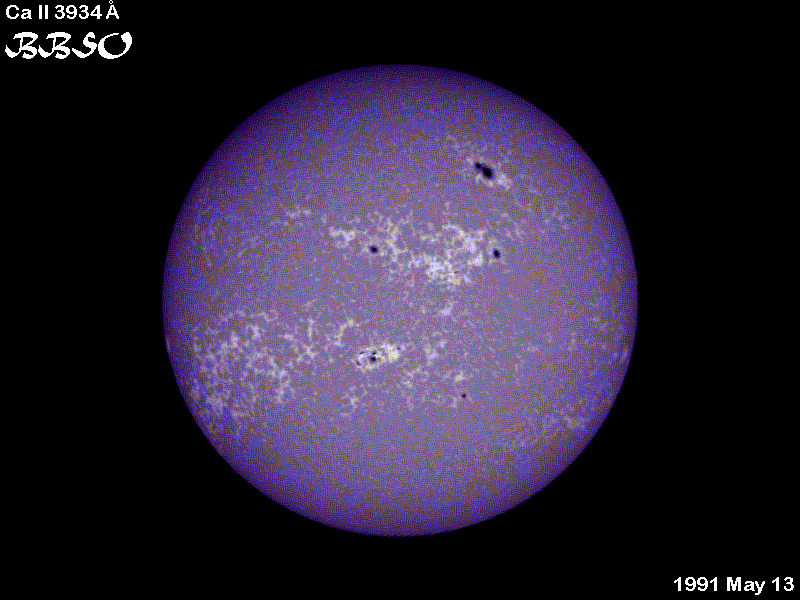
\includegraphics[scale=0.3]{CAII3934}
\label{fig:chromosphericnet}
\end{figure}

%En la figura \ref{fig:chromosphericnet} se observa una imagen tomada en la l\'inea de c\'alcio de la red cromosf\'erica, mientras que en la figura 

En a\~nadidura, las recientes observaciones del experimento VAULT (Very high Angular resolution ULtraviolet Telescope por sus siglas en ingl\'es) complementan la evidencia de una estructura ca\'otica cromosf\'erica y de la existencia de peque\~nos loops frios \cite{VAULT1}, los cu\'ales confirman la presencia de campos magn\'eticos.
VAULT es un proyecto de exploraci\'on espacial que data de 1999 y que busca estudiar la conexi\'on entre la corona y la crom\'osfera solar al observar la l\'inea espectral m\'as fuerte del sol, la Ly$\alpha$ a 1216A.
La resoluci\'on angular de subarcosegundos ($\approx$.3") permite ver directamente estructuras de la estructura de Sol Quieto. El parecido de los resultados entre los modelos y las observaciones indican que la explicaci\'on de las estructuras finas observadas en t\'erminos de loops frios es plausible.

Como se muestra en la figura x CORREGIR las im\'agenes de vault nos permiten mejorar la calidad de nuestras observaciones, permiti\'endonos tener un mejor entendimiento de la composici\'on de la atm\'osfera solar (n\'otese tambi\'en la calidad de la figura Y).

\begin{figure}[h]
\caption{"Fuente: Vourlidas, et al., 2009"}
\centering
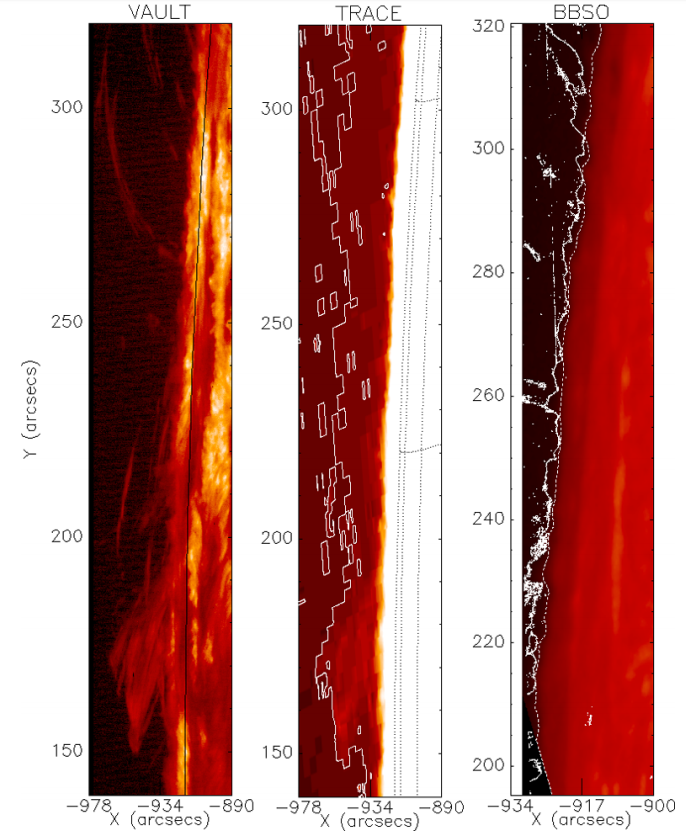
\includegraphics[scale=0.6]{vault_comparison}
\label{fig:vault_compare}
\end{figure}

\begin{figure}[h]
\caption{"Fuente: Vourlidas, et al., 2009}
\centering
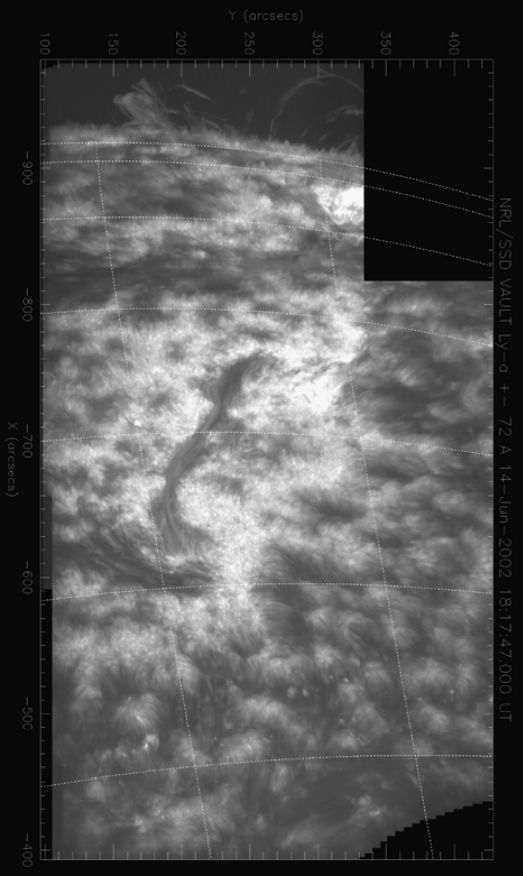
\includegraphics[scale=0.6]{vault_complete}
\label{fig:vault_complete}
\end{figure}



\section{El c\'odigo \emph{PakalMPI}}
%Descripci\'on del c\'odigo, puntualmente hay qu\'e explicar primero para qu\'e sirve actualmente y a partir de ello, plantear las modificaciones.
Como se mencion\'o anteriormente, esta tesis busca extender el c\'odigo PakalMPI. Este programa fue constru\'ido por Victor de la Luz en el a\~no 2011\cite{PAKAL}. Dicho programa es un modelo num\'erico inovador que pretende resolver la ecuaci\'on de transferencia radiativa en una geometr\'ia tridimensional (3D), usando una aproximaci\'on para una atm\'osfera localmente plano paralelo; lo anterior utilizando un sistema inteligente. Con este programa se generan las capas estratificadas de la atm\'osfera en una estructura l\'ogica. La salida del c\'odigo puede ser en forma de mapas bi-dimensionales o un perfil de una dimensi\'on, que reproduce las observaciones con alta presici\'on, dando informaci\'on f\'isica detallada acerca del entorno donde la radiaci\'on fue generada y/o transmitida.

Pakal se encuentra dividido en cuatro distintos m\'odulos: El modelo num\'erico, la geometr\'ia, los m\'etodos num\'ericos y las funciones f\'isicas. Estos cuatro m\'odulos pueden ser modificados independientemente sin afectar el funcionamiento de los otros. En esta tesis se modifica el m\'odulo de las funciones f\'isicas donde se resuelve la ecuaci\'on de transferencia.

Como todo modelo, PakalMPI est\'a basado en una serie de supuestos que le brindan una serie de fortalezas, pero tambi\'en una serie de limitantes; las cuales se presentar\'an a continuaci\'on. Con relaci\'n a sus supuestos, PakalMPI presenta un modelo aplicado a una geometr\'ia solar radial 3D, asumiendo una atm\'osfera local plano-paralela, y una emisi\'on t\'ermica de radio libre-libre de gas hidr\'ogeno-helio en equilibrio termodin\'amico. Adem\'as tambi\'en utiliza perfiles radiativos precalculados de densidad y temperatura (basado en modelos hidrost\'aticos, hidrodin\'amicos o MHD) para calcular la emisi\'on de una fuente de estructuras 3D con alta resoluci\'on espacial. En todo momento PakalMPI asume un estado de Sol Quieto y la ausencia de campos magn\'eticos. El t\'ermino Sol Quieto hace referencia a regiones del Sol que se encuentran exentas de cualquier manifestaci\'on de actividad observable. Con los supuestos antes mencionados, el programa concerniente resuelve la ecuaci\'on de transferencia radiativa en un conjunto de l\'ineas dirigidas de la fuente al observador.

En relaci\'on con las limitaciones de PakalMPI, si bien este permite la entrada de observaciones, no est\'a basado en ellas, y por lo tanto los resultados que no representan por completo las caracter\'isticas f\'isicas. De igual forma, PakalMPI se encuentra limitado a la fot\'osfera y crom\'osfera, esto debido a que estas regiones presentan una baja actividad magn\'etica lo cu\'al permite despeciarla; contrario a lo que ocurrir\'ia en la corona solar. PakalMPI tambi\'en omite la emisi\'on \emph{gyrosynchrotron} al despreciar los campos magn\'eticos. Finalmente, el c\'odigo de PakalMPI no logra reproducir en un 100\% las funci\'ones de densidad y temperatura del plasma solar.
 

En relaci\'on con sus fortalezas, 
Pakal puede mejorar la el tiempo de integraci\'on hasta por un orden de magnitud comparado a c\'odigos de integraci\'on lineal.
Pakal puede correr en clusters, supercomputadoras y computadoras personales con multiprocesadores, e incluso con computadoras personales convencionales.
Pakal permite modelar computacionalmente modelos emp\'iricos, te\'oricos y semi emp\'iricos, actualmente son usados modelos semi-emp\'iricos.
Modelos emp\'iricos: Aquellos que solo ajustan los perfiles a las observaciones sin tener ninguna base te\'orica para su desarrollo
Modelos te\'oricos: Aquellos que toman en cuenta \'unicamente las propiedades te\'oricas con las que contar\'ia un sistema como la Crom\'osfera.
Modelos semi-emp\'iricos: Son modelos te\'oricos con variables libres que se hacen ajustar a las observaciones.
Utilizando 32 procesadores de una m\'aquina Cray del CNS en san Luis Potos\'i, se ha podido generar espectros sint\'eticos de 32 frecuencias, con pasos de integraci\'on de 1km del centro del disco solar en aproximadamente 3 segundos.
Pruebas de convergencia y estabilidad de la parte num\'erica y del sistema experto fueron presentadas en De la Luz et al. (2010)

Mi modelo considera los campos magn\'eticos y por consiguiente una parte de la emisi\'on sincrotron. Este modelo extiende el modelo hidrodin\'amico de PakalPMI a un modelo magnetohidrodin\'amico, lo cu\'al es un poco m\'as acercado a la constituci\'on f\'isica de la crom\'osfera solar

Debido a las observaciones de espiculas es que se decidi\'o considerar el modelo de flujo emergente

Qu\'e es:


limitaciones



fortalezas
 

supuestos

Cuando los electrones individuales son desviados por un campo el\'ectrico producido por alg\'un ion, la aceleraci\'on pruducto de su cambio de trayectoria general emisi\'on Bremmstrahlung o libre-libre.  Para la emisi\'on en radio, los encuentros distantes con los iones son los m\'as comunes e importantes. Estos encuentros generan solo peque\~as desviaciones en su trayectoria. Los encuentros cercanos son menos probables, por lo que su contribuci\'on a la emisi\'on es mucho menor, adem\'as de producir grandes cambios de trayectorias.
Los par\'ametros de temperatura, densidad y de presi\'on son muy dif\'iciles de calcular, por lo que es una buena idea tomar los valores ya publicados. Sin embargo, no existe un solo modelo que vaya desde la Fot\'osfera hasta la Corona, debido principalmente a la complejidad que involucra tratar la zona de transici\'on. Adem\'as de que los procesos f\'isicos que trancurren en cada una de estas zonas difieren demasiado, por lo que es imposible manejar todo con un solo modelo.


Pakal lee la estructura atmosf\'erica, para lo cu\'al busca 5 perfiles fundamentales en funci\'on de la altura sobre la Fot\'osfera: temperatura, densidad de hidr\'ogeno, \'atomos presentes y el par\'ametro b1. Con estos valores se generan en una estructura l\'ogica las capas estratificadas de la atm\'osfera. A cada capa atmosf\'erica le corresponde un identificador. Este identificador es un valor de referencia para relacionar la metalicidad de cada capa. Como en principio sabemos cuales son los \'atomos presentes en cada capa, lo qeu necesitamos saber es la cantidad de ellos. Para eso se utiliza un modelo at\'omico ya provisto con los valores fundamentales, como sus potenciales de ionizaci\'on energ\'eticos. Adem





\chapter{Emisi\'on submilim\'etrica solar}
Mecanismos de la emisi\'on milim\'etrica del plasma del sol quieto, antecedente hist\'orico y enfoque del problema a resolver (qu\'e se va a hacer, por qu\'e se va a hacer y c\'omo se va a a hacer)

Estos mecanismos consisten en transiciones at\'omicas (que pueden ser ionizantes, de recombinaci\'on y tipo ligado-ligado) y mecanismos de emisi\'on libre-libre como radiaci\'on \emph{bremsstrahlung} y radiaci\'on sincrotr\'onica.

  
\chapter{Modelo de Micro estrucras magneticas solares}
\section{Caracteristicas Fisicas}

La base de la crom\'osfera presenta gr\'anulos con una escala de tama\~no relativamente mayor que aquellos presentes en la fot\'osfera concentrando flujo magn\'etico, el cual est\'a asociado con flujos verticales de plasma llamados \emph{esp\'iculas}. M\'as all\'a de la base de la crom\'osfera cambia la condici\'on en la presi\'on dominante, ya que mientras la presi\'on del gas domina a niveles fotosfericos, a estos niveles esta condici\'on se invierte y las distribuciones de brillo observadas est\'an dominadas por la geometr\'ia del campo magn\'etico.

La \emph{fot\'osfera}  consiste en granulos convectivos de peque\~na escala ($10^3$~km), separados de entre s\'i por capas intergranulares, las cuales concentran elementos de alto flujo magn\'etico ($|B| \le 1\mbox{kG}$). La escala temporal de la ocurrencia de un gr\'anulo es de unos minutos aproximadamente.



Aqui van las propiedades fisicas de los modelos que vamos a implementar. Por ejemplo, definir las escalas de altura, las intensidades de campo, temperatura, densidades, etc.

Para llevar a cabo la simulaci\'on del comportamiento de los campos magn\'eticos se utilizaron dos modelos distintos; uno en forma de arcos magn\'eticos \cite{loops} y otro en forma de un flujo emergente \cite{flujoemergente}.

La primer aproximaci\'on para el modelo de campo magn\'etico fue el de un loop con forma semi-circular, el cu\'al puede ser modelado como un campo magn\'etico dipolo generado por un cable dipolo enterrado debajo de la fo\'sfera.
En este modelo es posible calcular las tres componentes del campo magn\'etico por medio de las siguientes ecuaciones \citation{Jackson}:

\begin{equation}
    B_r(r,\theta)=\frac{2mcos\theta}{r^3}
\end{equation}
  
\begin{equation}
    B_\theta(r,\theta)=\frac{2msin\theta}{r^3}
\end{equation}

\begin{equation}
    B_\phi(r,\theta)=0
\end{equation}

Donde m representa el momento magn\'etico inducido por el anillo de corriente I con un conductor de radio a, y los par\'ametros theta y r son los par\'ametros libres que movemos para ir generando los valores del campo.

Para la segunda aproximaci\'on del modelo se consider\'o un flujo emergente, ya que una gran cantidad del flujo magn\'etico en la fot\'osfera solar consiste en fuertes campos en elementos no resueltos. Este modelo consiste en un elemento magn\'etico con una simetr\'ia de un tubo de flujo cil\'indrico incrustado en la fot\'osfera.

Los valores de sus componentes son calculados como

\begin{equation}
B_z(r,z)=B_z(0,z)D(\alpha)
\end{equation}

\begin{equation}
B_r(r,z)=-\frac{1}{2}r\frac{dB_z(0,z)}{dz}D(\alpha)
\end{equation}

Este campo satisface gradiente $ \nabla \cdot B = 0 $. La funci\'on radial $D(\alpha)$ es tomada como
\begin{equation}
 D(\alpha) = 
    \begin{cases}
        (1-alpha^2)^2 & \alpha \leq 1 \\
        0   & \alpha > 1
    \end{cases}
\end{equation}

donde $\alpha = r/r_0(z)$. El radio $r_0(z)$ del tubo a una altura z es promediado a lo largo del c\'irculo de radio R que es obtenido de:

\begin{equation} \label{r_flujo_emergente}
r_0^-2(z) = \frac{2\pi B_z(0,z)}{\phi} \int_{0}^{1} \alpha D(\alpha) d\alpha = \frac{\pi B_z(0,z)}{3 \phi}
\end{equation}

donde $\phi$ es el flujo magn\'etico dentro del tubo.
El campo axial es considerado

\begin{equation}
B_z(0,z)=B_0e^{\frac{-z}{h}}
\end{equation}

Por lo tanto la fuerza axial de campo es $B_0$ en el origen $z=0$ que en nuestro caso se ubica al nivel de la fot\'osfera (CORRIGEME). En este modelo el campo diverge a diferente ritmo dependiendo de la escala de altura h.

Conforme $h\rightarrow \infty , B_z(0,z) \rightarrow B_0$, $a$ constante, y por la ecuaci\'on \ref{r_flujo_emergente} $r_0(z) \rightarrow r_0 = (3\phi / \pi B_0)^\frac{1}{2}$, es tambi\'en una constante.

En los c\'alculos consideramos $\phi=2.8x10^18$Mx y $B0=2000$Gauss. Esto implica tubos de flujo de 366km a $Z=0$


\section{Implementaci\'on del modulo para Magnetohidrost\'atica}
Aqui va la info de como implementaste los modelos.


\chapter{Resultados}
\section{Micro arco magnetico}
resultados de las simulaciones para el modelo de arcos magneticos
\section{Flujo emergente}
resultados de las simulaciones para flujo emergente


\chapter{Discusi\'on y conclusiones}
Comparaci\'on entre ambos modelos, discusion y resultados
hola Springer Science \& Business Media, Aug 26, 2006

\begin{thebibliography}{9}

\bibitem{carrington} 
Robert D. Loper
\textit{Carrington-class events as a great filter for electronic civilizations in the drake equation} 
Astronomical Society of the Pacific, 2019.

\bibitem{VAULT1} 
A. Vourlidas, B. Sanchez, E. Landi, et al.
\textit{The structure and Dynamics of the Upper Chromosphere and Lower Transition Region as Revealed by the Subarcsecond VAULT Observations, Astronomy and Astrophysics} 
Solar Physics, 2010.

\bibitem{VALC}
J. E. Vernazza, E. H. Avrett y R. Loeser
\textit{Structure of the Solar Chromosphere. III. Models of the EUV Brightness Components of the Quiet Sun} 
The Astrophysical Journal Supplement Series, 1981.

\bibitem{C7}
J. M. Fontenla, E. H. Avrett y R. Loeser
\textit{Energy Balance in the Solar Transition Region. I. Hydrostatic Thermal Models with Ambipolar Difussion} 
The Astrophysical Journal, 1990.

\bibitem{PAKAL}
V. de la Luz
\textit{Modelaci\'on Tridimensional de la Atm\'osfera Solar para el Estudio de su Emisi\'on en Radio} 
2011.

\bibitem{loops} 
Markus Aschwanden. 
\textit{Physics of the Solar Corona} 
Springer Science \& Business Media, 2006.

\bibitem{flujoemergente} 
Rees and Seemel.
\textit{Line Formation in an Unresolved Magnetic Element: A Test of the Centre of Gravity Method} 
Astronomy and Astrophysics, 1978

\bibitem{Jackson} 
A. Vourlidas, B. Sanchez, E. Landi, et al.
\textit{Classical Electrodynamics} 
John Wiley and Sons, 1962.

\bibitem{NASAweb} 
Hathaway, D.
\textit{Chromospheric Features} 
https://solarscience.msfc.nasa.gov/feature2.shtml, NASA, 2014.

\bibitem{chromotemp} 
Fleishman G and Melnikov V
\textit{Gyrosynchrotron emission from anisotropic electron distributions} 
The Astrophysical Journal, 2003

\end{thebibliography}




\end{document}    </include>
    </context>

    <context id="math-2" style-ref="math" class="no-spell-check">
      <start>\\\[</start>
      <end>\\\]</end>
      <include>
        <context sub-pattern="0" where="start" style-ref="math-boundary"/>
        <context sub-pattern="0" where="end" style-ref="math-boundary"/>
        <context ref="in-math"/>
      </include>
    </context>

    <context id="math-env" style-ref="math" style-inside="true" class="no-spell-check">
      <start>(\\begin)\{(math|displaymath|equation\*?|align\*?|eqnarray\*?)\}</start>
      <end>(\\end)\{\%{2@start}\}</end>
      <include>
        <context sub-pattern="1" where="start" style-ref="common-commands"/>
        <context sub-pattern="1" where="end" style-ref="common-commands"/>
        <context ref="in-math"/>
      </include>
    </context>

    <context id="inline-math-1" style-ref="inline-math" class="no-spell-check">
      <start>\$</start>
      <end>\$</end>
      <include>
        <context sub-pattern="0" where="start" style-ref="math-boundary"/>
        <context sub-pattern="0" where="end" style-ref="math-boundary"/>
        <context ref="in-math"/>
      </include>
    </context>

    <context id="inline-math-2" style-ref="inline-math" class="no-spell-check">
      <start>\\\(</start>
      <end>\\\)</end>
      <include>
        <context sub-pattern="0" where="start" style-ref="math-boundary"/>
        <context sub-pattern="0" where="end" style-ref="math-boundary"/>
        <context ref="in-math"/>
      </include>
    </context>

    <context id="math">
      <include>
        <context ref="math-1"/>
        <context ref="math-2"/>
        <context ref="math-env"/>
        <context ref="inline-math-1"/>
        <context ref="inline-math-2"/>
      </include>
    </context>

    <context id="latex">
      <include>
        <context ref="comment"/>
        <context ref="verbatim"/>
        <context ref="R-block"/>
        <context ref="headings"/>
        <context ref="math"/>
        <context ref="urls"/>
        <context ref="specific-commands"/>
        <context ref="common-commands"/>
        <context ref="special-char"/>
        <context ref="gen
